Dans l'ensemble de ce rapport, jusqu'à maintenant, nous considérions tout particulièrement la banque d'images MNIST en tant que jeu de données d'entraînement des réseaux étudiés. Il s'agit d'un jeu composé de 70000 images digitales en niveaux de gris, échelonnées entre 0 et 1 et de taille 28x28 pixels, représentant des digits (chiffres) écrits à la main \cite{LeCun_2005}. Les objets sur les images (ensemble des pixels de valeurs strictement positives, qui se détache visuellement du fond de l'image, dont les valeurs sont proches de 0) de ce jeu de données sont particulièrement fins, et peuvent être considérés topologiquement comme des filaments entrelacés. Cet aspect-là rend ce jeu très spécifique dans le cadre d'opérations morphologiques, et peut donner sur les réseaux morphologiques étudiés des résultats bien particuliers. \\

\vspace{-1.2mm}
\noindent L'ensemble des expériences citées durant ce rapport a également été réalisé, en parallèle de MNIST, avec un autre jeu de données : FashionMNIST. Il s'agit d'une banque de 70000 images digitales en niveaux de gris, échelonnées entre 0 et 1 et de taille 28x28 pixels également, mais qui représente cette fois-ci des vêtements de tout type (pantalons, chemises, robes, etc.). Contrairement à MNIST, ce jeu de données représente donc des objets bien plus larges et imposants face au support des images, et les résultats d'entraînement des réseaux morphologiques avec un tel jeu peuvent être bien différents de ceux avec MNIST. \\

\vspace{-1.2mm}
\noindent La figure suivante (\ref{fig:mnist_and_fashionmnist}) permet de visualiser une partie des images des deux banques MNIST (\ref{fig:sum1}) et FashionMNIST (\ref{fig:sum2}). \\

%figure
\vspace{-0.2mm}
\begin{figure}[ht]
  \begin{center}
      \subfigure[MNIST]{
          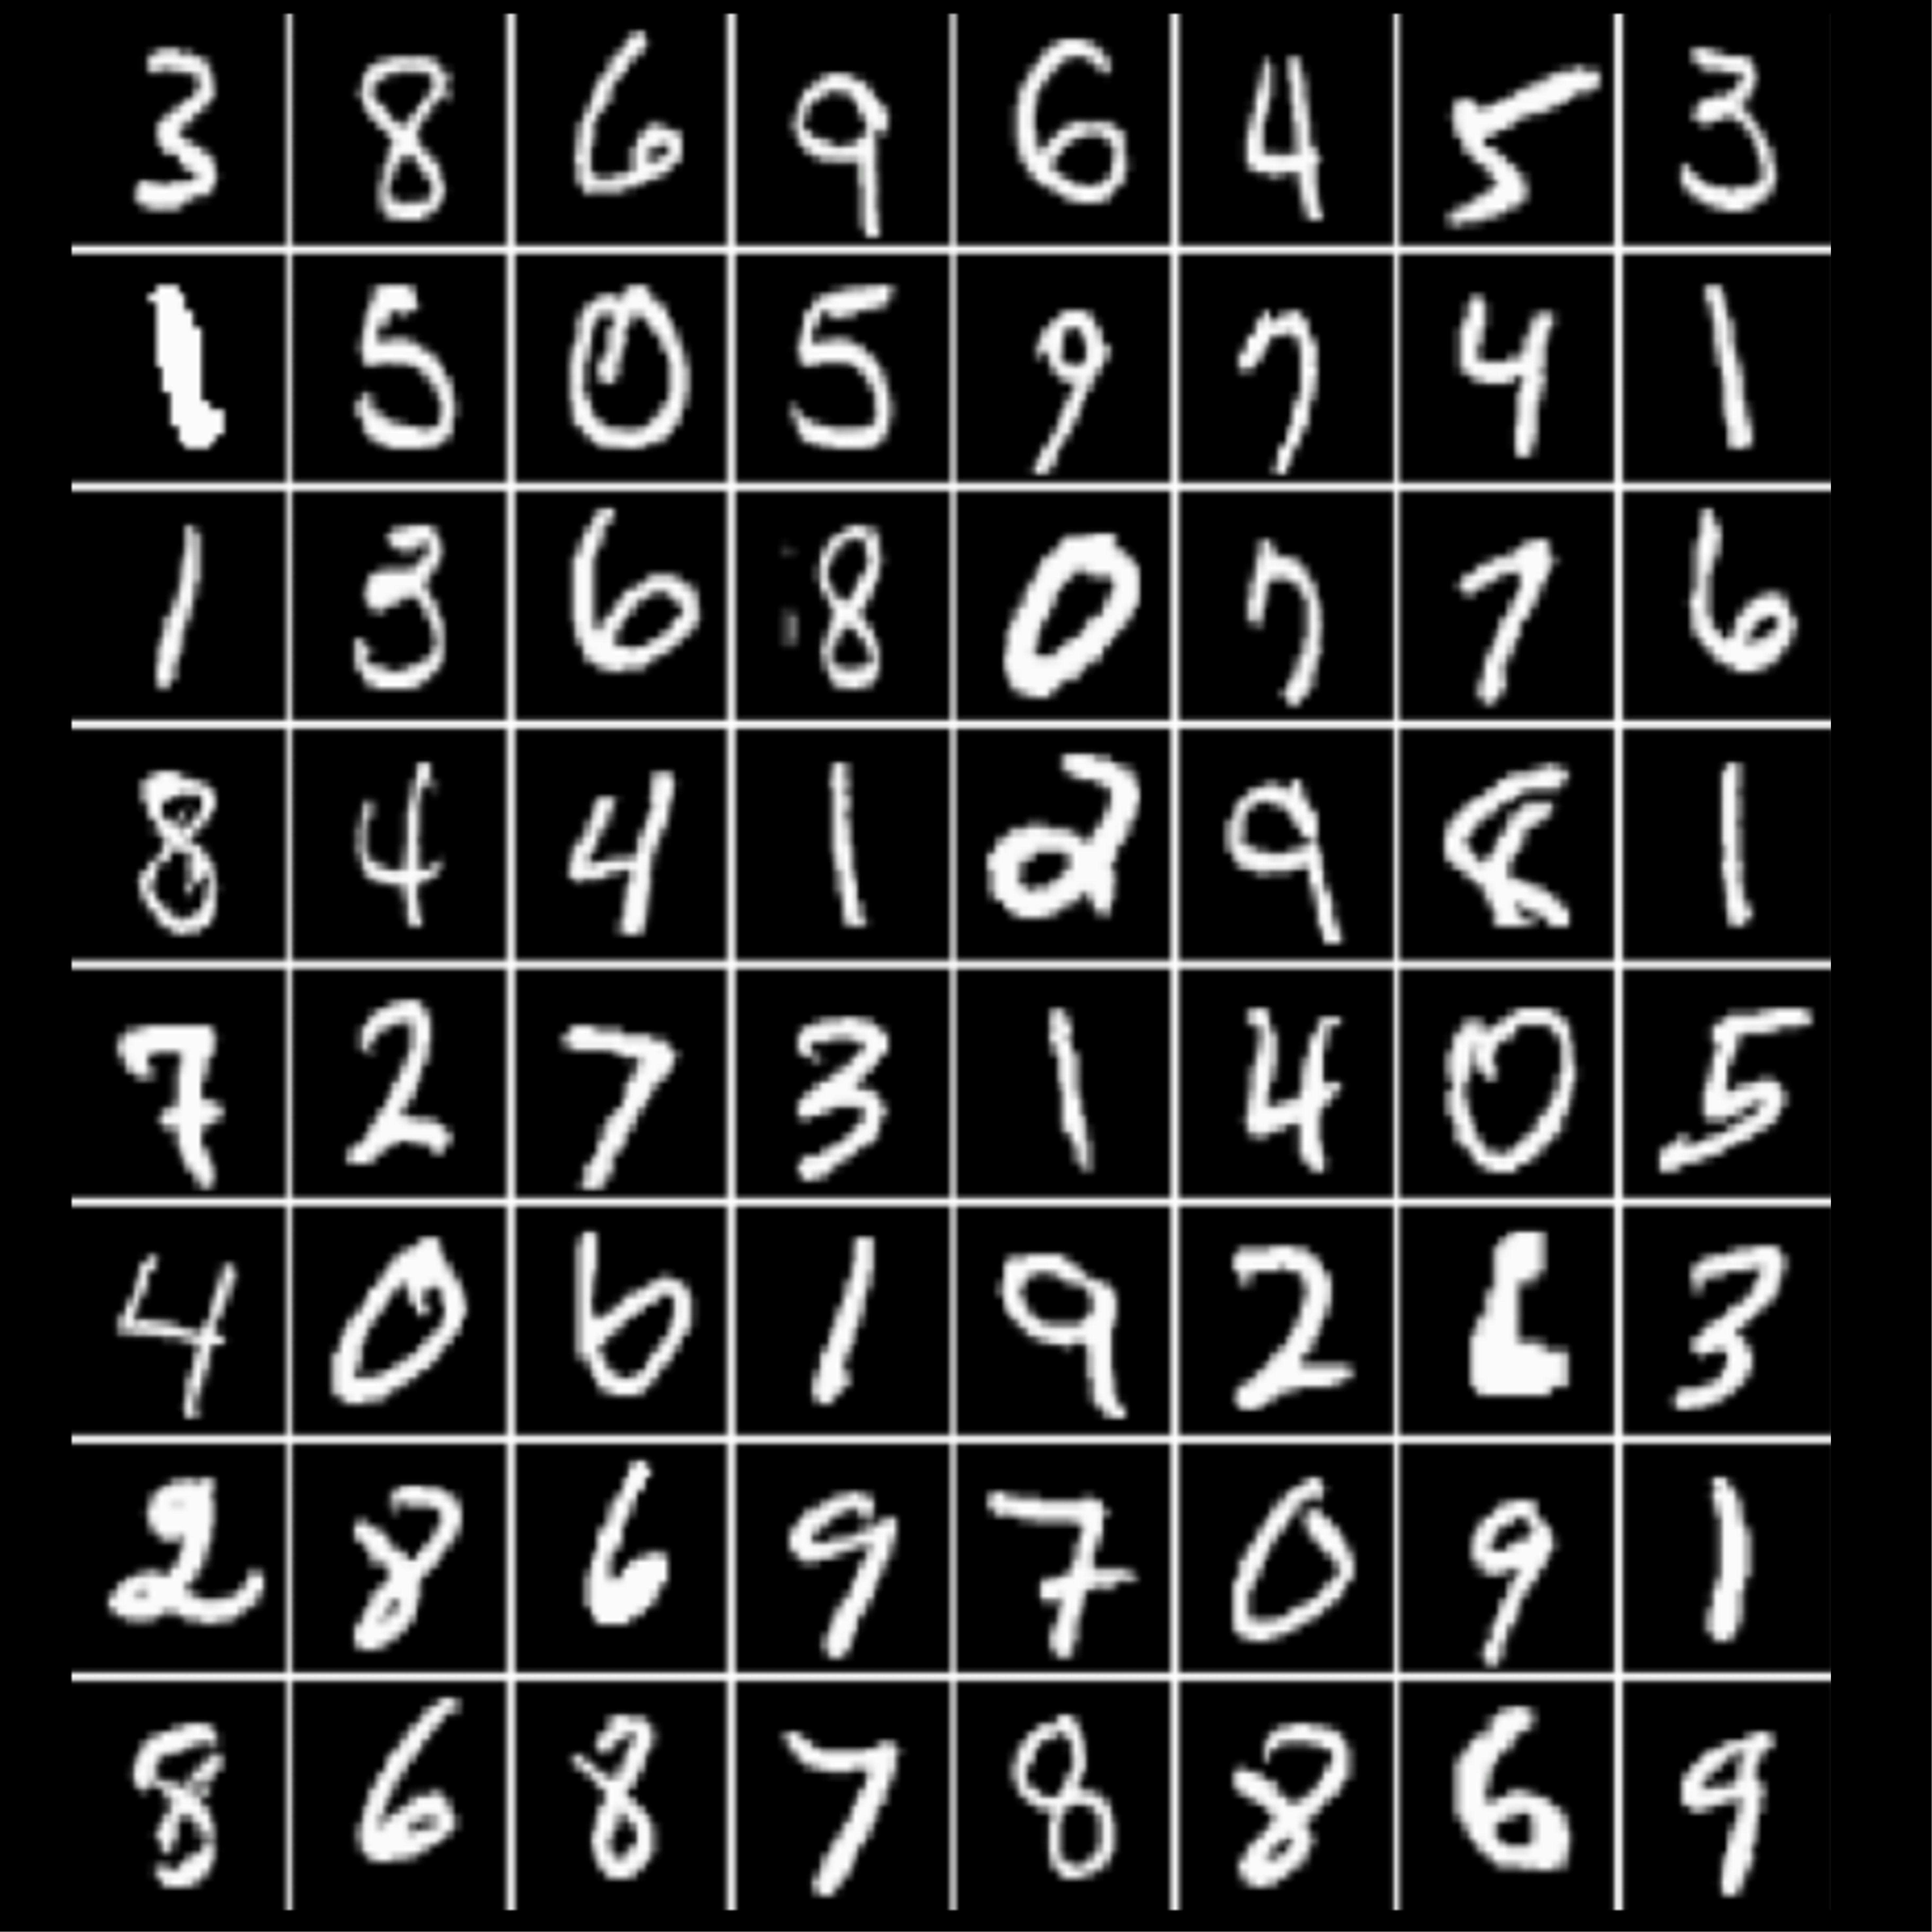
\includegraphics[width=0.24\textwidth]{parts/4-analyse_des_reseaux/impact_database/figures/ill_mnist.pdf}
          \label{fig:sum1}}
      \hspace{12.0mm}
      \subfigure[FashionMNIST]{
          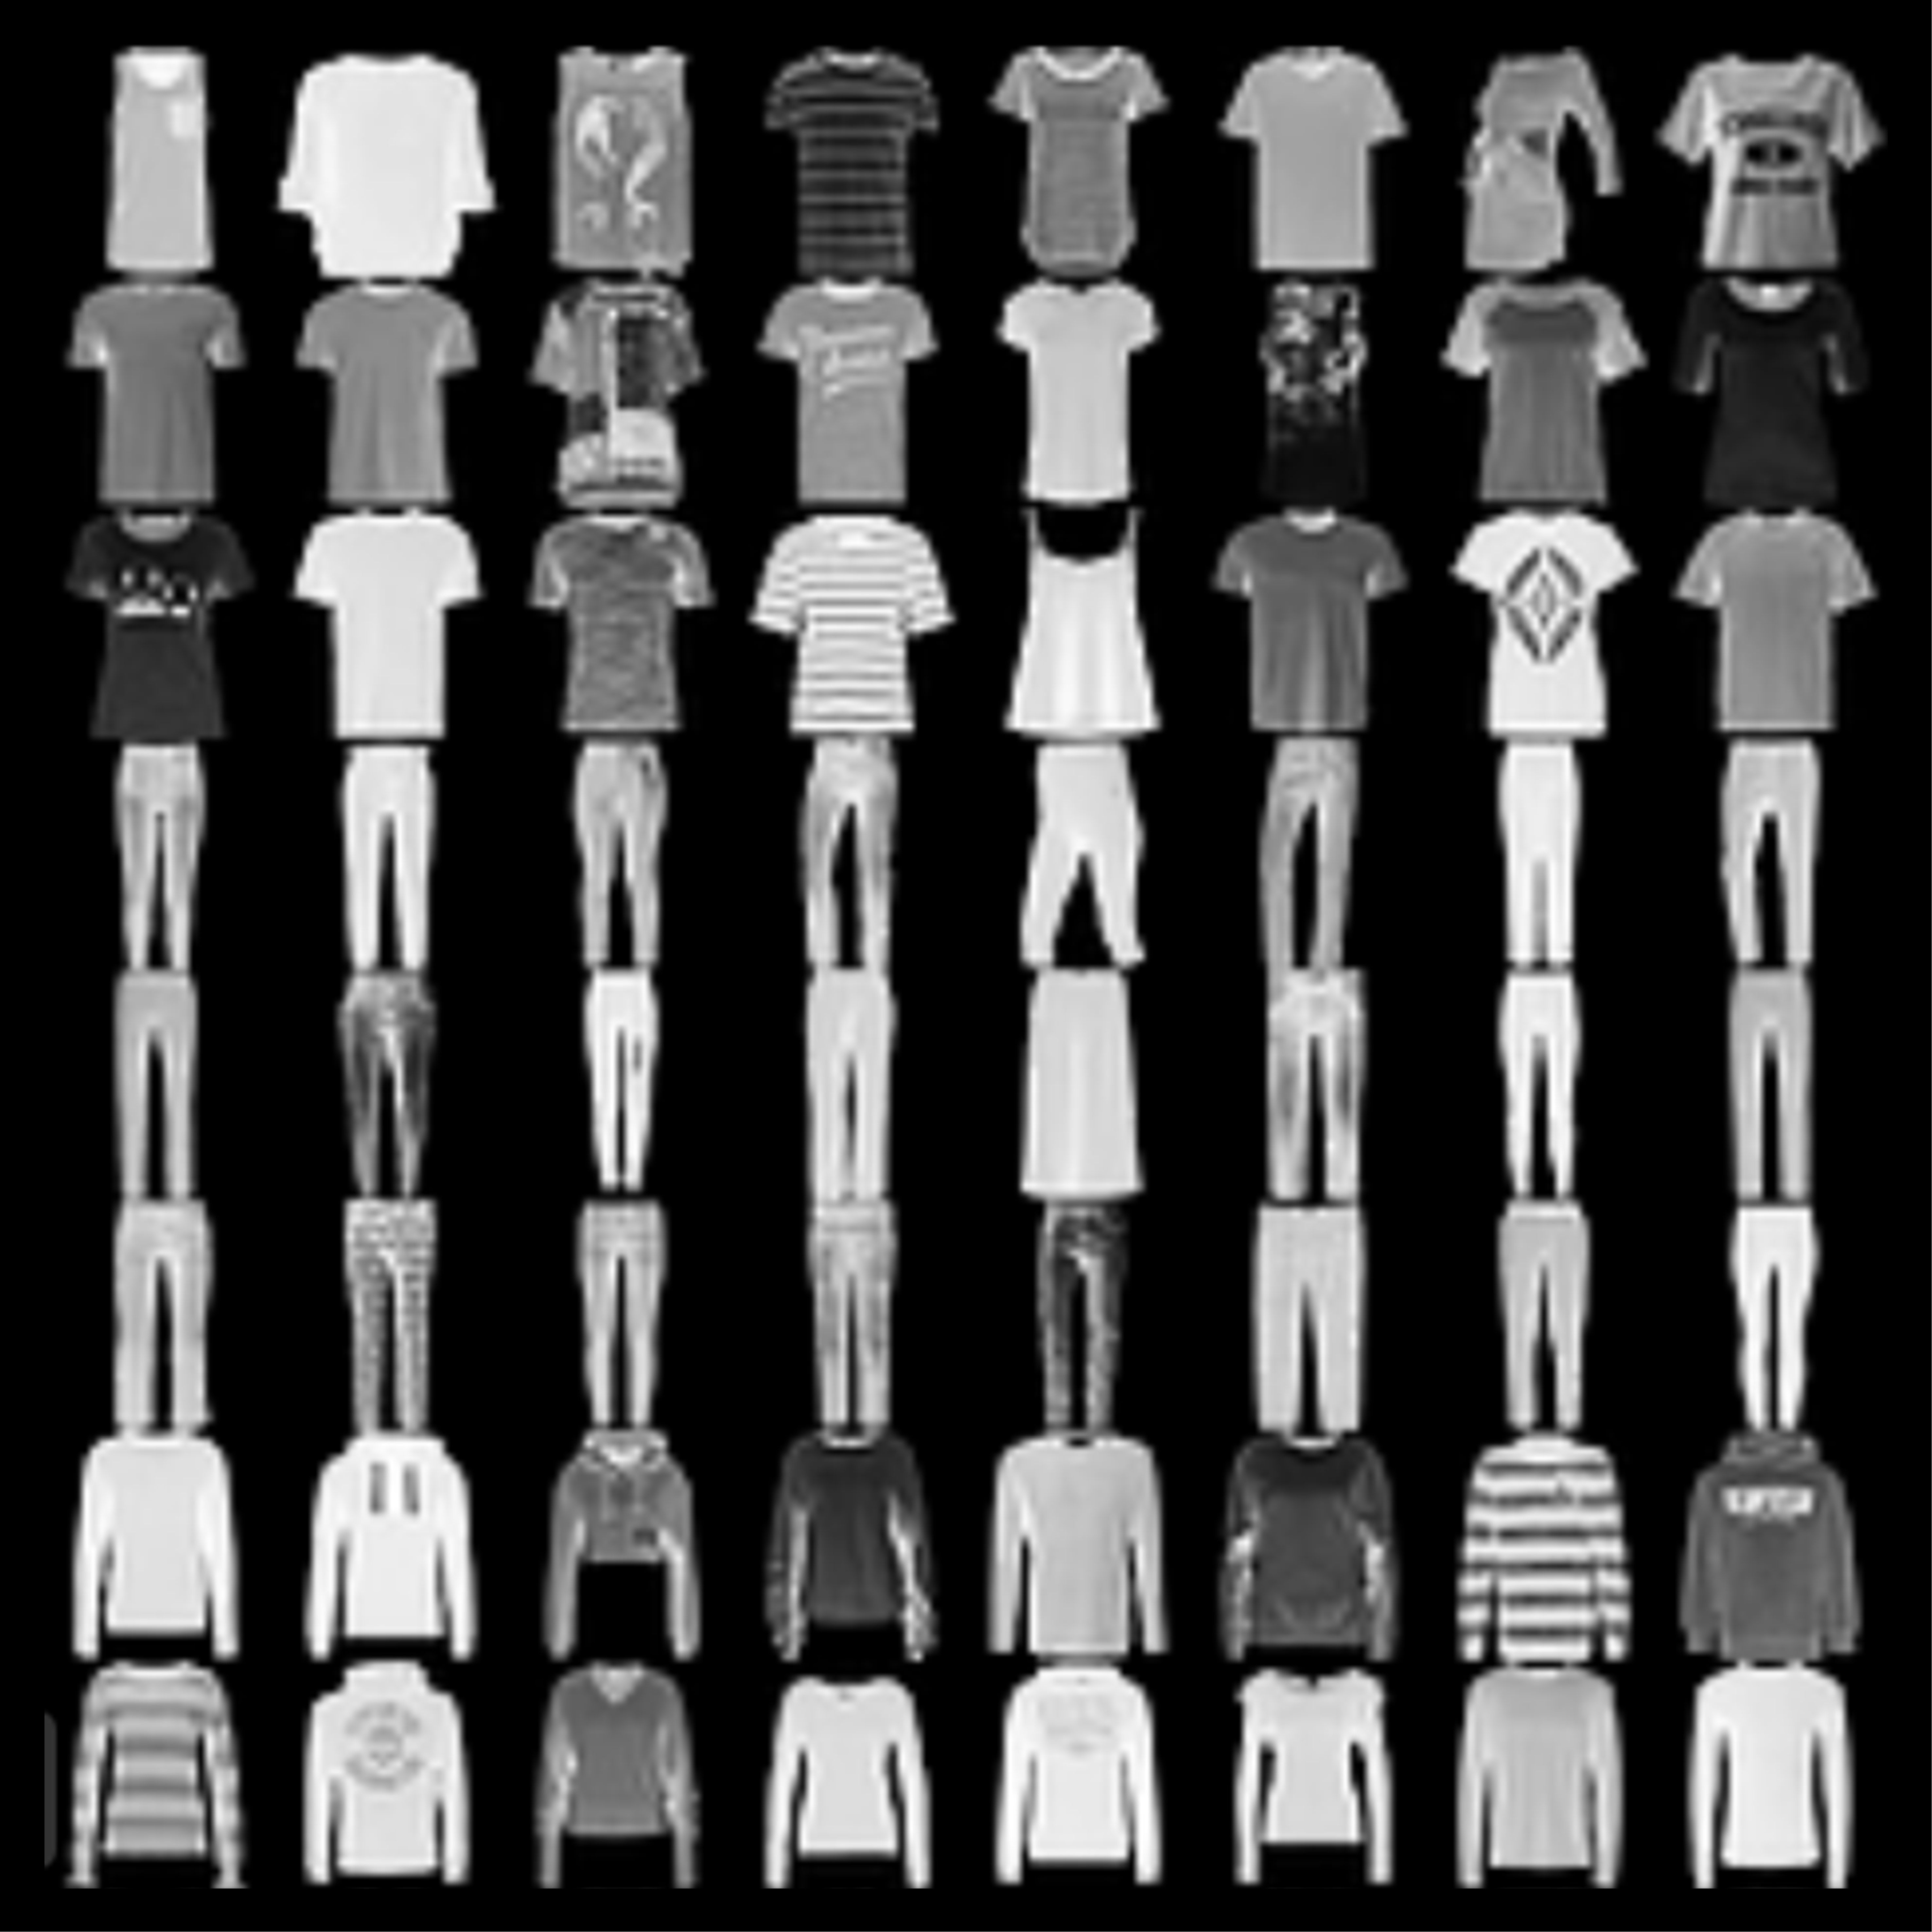
\includegraphics[width=0.24\linewidth]{parts/4-analyse_des_reseaux/impact_database/figures/ill_fashionmnist.pdf}
          \label{fig:sum2}}
    \vspace{-0.1mm}
    \caption{ \centering Echantillon des jeux de données MNIST (\ref{fig:sum1}) et FashionMNIST (\ref{fig:sum2}).}
    \label{fig:mnist_and_fashionmnist}
  \end{center}
\end{figure}

\vspace{-3.2mm}
Le but est alors de comparer les résultats de convergence d'un même réseau pour les même expériences entre ces deux jeux de données MNIST et FashionMNIST, et ainsi mieux comprendre leur impact sur la convergence des réseaux morphologiques.
